\documentclass[11pt,a4paper]{article}
\usepackage[margin=26mm]{geometry}
\usepackage[T1]{fontenc}
\usepackage{lmodern,microtype}
\usepackage{amsmath,amssymb,amsthm,mathtools,booktabs,array,longtable}
\usepackage{tikz}
\usepackage[colorlinks=true,linkcolor=blue,citecolor=blue,urlcolor=blue]{hyperref}
\setlength{\emergencystretch}{1em}
\hypersetup{pdftitle={Structural refinements and formal certificates for C7 and C13 zero-error codes}}
\newtheorem{theorem}{Theorem}[section]
\newtheorem{lemma}[theorem]{Lemma}
\newtheorem{proposition}[theorem]{Proposition}
\newtheorem{corollary}[theorem]{Corollary}
\theoremstyle{definition}
\newtheorem{definition}[theorem]{Definition}
\theoremstyle{remark}
\newtheorem{remark}[theorem]{Remark}
\newcommand{\Z}{\mathbb Z}
\newcommand{\N}{\mathbb N}
\newcommand{\conf}{\mathrel{\simeq}}
\newcommand{\sep}{\mathrel{\perp}}
\newcommand{\Nb}{\mathcal N}
\newcommand{\Gao}{\operatorname{Gao}}
\newcommand{\Het}{\operatorname{Het}}
\newcommand{\PhiG}{\Phi}
\newcommand{\dd}{\mathrm d}
\newcommand{\code}[1]{\texttt{\detokenize{#1}}}
\title{Structural refinements and formal certificates\protect\\
for $C_7$ and $C_{13}$ zero-error codes}
\author{}
\date{4 October 2026}
\begin{document}
\maketitle
\begin{abstract}
We study simultaneous mask allocation on three actual fibers of a strong power
of the thirteen-cycle. For a center of prescribed size $a$ and two leaves of
required sizes at least $b,c$, the pairwise budgets $a+b,a+c\le169$ do not
characterize feasibility. In the small-slack regime
$u=169-a-b<13$, $v=169-a-c<13$, the exact additional condition is
$\min(a,169-a)\le uv$. A minority-rectangle argument proves necessity for
arbitrary masks; a Ferrers diagram or its complement proves sufficiency.
The result is realized in $C_{13}^{\boxtimes6}$ and formalized in Lean,
including the sharp balanced occupancy $80$ and a $240$-point example.
For context we publish complete formal certificates for the existing bounds
$\Theta(C_7)>3.258834805519757$ and
$\Theta(C_{13})>6.302927403571109$, obtained within inherited recursive and
guarded-cell methods. An appendix gives a classical correlated $C_7^3$
illustration with full coordinate margins. The local theorem and that
illustration do not improve these capacity bounds.
\end{abstract}

\section{Scope, notation and construction context}
Let $C_q$ be the cycle on $\Z/q\Z$. Its closed confusability relation is
$x\conf y$ when $x-y\in\{0,1,-1\}$. On a strong power, two words are
confusable exactly when they are confusable in every coordinate. A zero-error
code is a finite set in which distinct words are not confusable, equivalently
an independent set of the strong power. We use
\[
 \Theta(G)=\sup_{d\ge1}\alpha(G^{\boxtimes d})^{1/d}.
\]
For sets $S,T$ write $S\sep T$ if no point of $S$ is confusable with a point
of $T$. This includes exclusion of equality. Write $\Nb(S)$ for the closed
neighborhood of $S$.

The main question here is structural: how can two different directional
separation requirements constrain a \emph{shared} center? Our answer is an exact
local region, not a new general coding framework. Its elementary proof is
self-contained. Ferrers compression and discrete isoperimetry are classical;
grid and torus inequalities of Bollob\'as--Leader provide relevant context
\cite{grid,torus}, but are not invoked as a theorem implying our allocation
formula. We do not assert worldwide priority for the elementary ingredients.

The capacity constructions placed alongside this result have a different
role. Gao isolated a recursive private-pair invariant \cite{gao};
Buys--Polak--Zuiddam (BPZ) supplied improved finite data, layered
substitutions and Lean certificates \cite{bpz,bpzcode}; Tandon enlarged the
auxiliary-set construction by one-sided heterogeneity \cite{tandon}.
Protti introduced guarded typed-cell refinements \cite{protti}, and Long
published improved recursion DAGs \cite{long}. The retained $C_7$ certificate
uses the Gao--BPZ--Tandon methods. The retained $C_{13}$ certificate is a new
concrete combination of Protti's guarded cells with Long's DAG, not the
invention of guarded cells. The local mask theorem below addresses a question
not answered by scalar pairwise size budgets in these constructions.

Table~\ref{tab:roots} compares \emph{chosen construction roots}, using
Stavriianov's C7 certificate~\cite{stav} and Long's C13 certificate~\cite{long}. These are
not the unknown capacities and no global optimality is asserted. All source
versions in the comparison are fixed, as identified in the references and
the companion's \code{NOTICE.md}.
\begin{table}[ht]
\centering\small
\begin{tabular}{@{}llll@{}}
\toprule
Cycle & Selected prior construction & Retained construction & Dimensions\\
\midrule
$C_7$ & Stavriianov: $3.258834362237710794\ldots$
      & $3.258834805519757\ldots$ & $560\,/\,300$\\
$C_{13}$ & Long: $6.302927071589786110\ldots$
      & $6.302927403571109071\ldots$ & $522\,/\,522$\\
\bottomrule
\end{tabular}
\caption{Prior and retained code roots, not equalities for $\Theta(C_q)$.
The structural round reported in this paper adds no capacity gain.}
\label{tab:roots}
\end{table}

The companion repository contains the paper, mathematical construction data,
and a portable, pinned Lean project. The single aggregate module
\code{StructuralRelease} exports aliases for both strict capacity endpoints,
the actual local region, the physical example and the $C_7$ illustration.
The argument proceeds from a combinatorial lemma to the exact region, then
to its graph realization; Sections~\ref{sec:capacity}--\ref{sec:formal} give
the contextual construction and certificate interfaces.

\section{A minority rectangle on a cyclic grid}
Consider a binary matrix $f:X\times Y\to\{0,1\}$ on finite sets.
A row $\{x\}\times Y$ is \emph{mixed} if both colors occur; a column
$X\times\{y\}$ is mixed in the analogous sense. Denote their index sets by
$R_f\subseteq X$ and $Q_f\subseteq Y$.

\begin{lemma}[Minority rectangle]\label{lem:minority}
If $|R_f|<|X|$ and $|Q_f|<|Y|$, one color occurs only in
$R_f\times Q_f$. In particular,
\[
 \min\bigl(|f^{-1}(1)|,|f^{-1}(0)|\bigr)\le |R_f|\,|Q_f|.
\]
\end{lemma}
\begin{proof}
Choose an unmixed row and an unmixed column. Their constant colors agree at
the intersection; call this color $\varepsilon$. Every unmixed row meets the
chosen unmixed column, so has color $\varepsilon$, and every unmixed column
meets the chosen unmixed row, so has that same color. A point of the other
color must therefore lie on both a mixed row and a mixed column. Counting
their intersections proves the inequality. Notice that the color singled
out by the argument need not be specified in advance.
\end{proof}

Set $H=(\Z/13\Z)^2$, $e_1=(1,0)$ and $e_2=(0,1)$. For $A\subseteq H$
define its two directional exit boundaries and their sizes by
\[
 \partial_i A=(A+e_i)\setminus A,
 \qquad d_i(A)=|\partial_i A| \quad (i=1,2).
\]
Thus $|A\cup(A+e_i)|=|A|+d_i(A)$. A mixed column, with the second
coordinate fixed, has at least one transition from membership to
nonmembership while cycling in direction $e_1$. These transitions occur
in distinct columns; consequently $|Q_A|\le d_1(A)$. Similarly
$|R_A|\le d_2(A)$.

\begin{proposition}[Directional minority bound]\label{prop:boundary}
For any $A\subseteq H$ with $d_1(A),d_2(A)<13$,
\begin{equation}\label{eq:minority}
 \min(|A|,169-|A|)\le d_1(A)d_2(A).
\end{equation}
\end{proposition}
\begin{proof}
The bounds on the mixed-line counts ensure an unmixed row and column.
Apply Lemma~\ref{lem:minority} to the indicator of $A$, then use
$|R_A|\le d_2(A)$ and $|Q_A|\le d_1(A)$.
\end{proof}

We will also use
\begin{equation}\label{eq:complement}
 d_i(H\setminus A)=d_i(A).
\end{equation}
On each cyclic line the number of $1\to0$ transitions equals the number of
$0\to1$ transitions, since every entry into a run must be followed by an
exit. Summing over the lines proves~\eqref{eq:complement}. This symmetry
explains why the smaller of a shape and its complement, rather than just
the center size, controls the region.

\section{The exact two-direction allocation region}
\begin{definition}[Compatible star masks]
Three subsets $A,B,C\subseteq H$ are compatible when
\begin{equation}\label{eq:compat}
 B\cap\bigl(A\cup(A+e_1)\bigr)=\varnothing,
 \qquad
 C\cap\bigl(A\cup(A+e_2)\bigr)=\varnothing.
\end{equation}
There is no constraint between $B$ and $C$. They occupy different leaves,
not a common physical fiber.
\end{definition}

\begin{theorem}[Exact small-slack region]\label{thm:region}
Let $a,b,c\in\N$ satisfy $a+b\le169$, $a+c\le169$, and put
\[
 u=169-a-b<13,\qquad v=169-a-c<13.
\]
There are compatible masks with \emph{exact} center size $|A|=a$ and
leaf sizes \emph{at least} $|B|\ge b$, $|C|\ge c$ if and only if
\begin{equation}\label{eq:region}
 \min(a,169-a)\le uv.
\end{equation}
\end{theorem}
\begin{proof}
Necessity follows from the two disjointness conditions:
\[
 a+d_1(A)+b\le169,\qquad a+d_2(A)+c\le169.
\]
Hence $d_1(A)\le u$, $d_2(A)\le v$. The strict upper bounds on $u,v$
allow Proposition~\ref{prop:boundary}, giving
$\min(a,169-a)\le d_1(A)d_2(A)\le uv$.

For sufficiency, first suppose $a\le uv$. Inside the nonwrapping rectangle
$\{0,\ldots,v-1\}\times\{0,\ldots,u-1\}$ choose the initial row-major
Ferrers diagram
\begin{equation}\label{eq:ferrers}
 F_{v,u}(a)=\{(x,y):0\le x<v,\ 0\le y<u,\ xu+y<a\}.
\end{equation}
It has exactly $a$ cells. In each occupied column its first-coordinate
section is an initial interval of length less than $13$, and in each
occupied row its second-coordinate section is likewise an initial
interval. Each nonempty section has one exit. Thus
$d_1(F_{v,u}(a))\le u$ and $d_2(F_{v,u}(a))\le v$.
If instead $169-a\le uv$, take $A=H\setminus F_{v,u}(169-a)$;
equation~\eqref{eq:complement} gives the same bounds and $|A|=a$.

In either case choose
\begin{equation}\label{eq:maxleaves}
 B=H\setminus\bigl(A\cup(A+e_1)\bigr),\qquad
 C=H\setminus\bigl(A\cup(A+e_2)\bigr).
\end{equation}
They are compatible and have sizes $169-a-d_1(A)\ge b$ and
$169-a-d_2(A)\ge c$. If $u=0$ or $v=0$, condition~\eqref{eq:region}
forces $a=0$ or $a=169$; the empty diagram or its full complement gives
the same conclusion, so no division by a zero rectangle width is needed.
\end{proof}

The theorem compares joint feasibility with scalar edge budgets. For
$(a,b,c)=(81,81,81)$ both pair sums are $162\le169$, but $u=v=7$ and
$\min(81,88)=81>49$. The requirements therefore cannot be realized.
This is a concrete obstruction even though each pairwise budget has slack.
The use of lower bounds on the leaves is intentional: the construction
takes the full dilation complements. A theorem imposing exact leaf
sizes would be a differently phrased statement, not the formal interface
used here.

\begin{corollary}[Sharp balanced occupancy]\label{cor:80}
Every compatible triple has
$\min(|A|,|B|,|C|)\le80$. Equality is attained.
\end{corollary}
\begin{proof}
If all three sizes are at least $81$, then $81\le a\le88$ and the
dilation budgets give $d_1(A),d_2(A)\le7$. Equation~\eqref{eq:minority}
would force $81\le49$, a contradiction. For equality, take
\[
 A=\{0,\ldots,8\}^2\setminus\{(8,8)\}
\]
and choose $B,C$ by~\eqref{eq:maxleaves}. Here $|A|=80$, each of its nine
occupied rows and nine occupied columns contributes exactly one exit,
and $|B|=|C|=169-80-9=80$.
\end{proof}

\begin{figure}[ht]
\centering
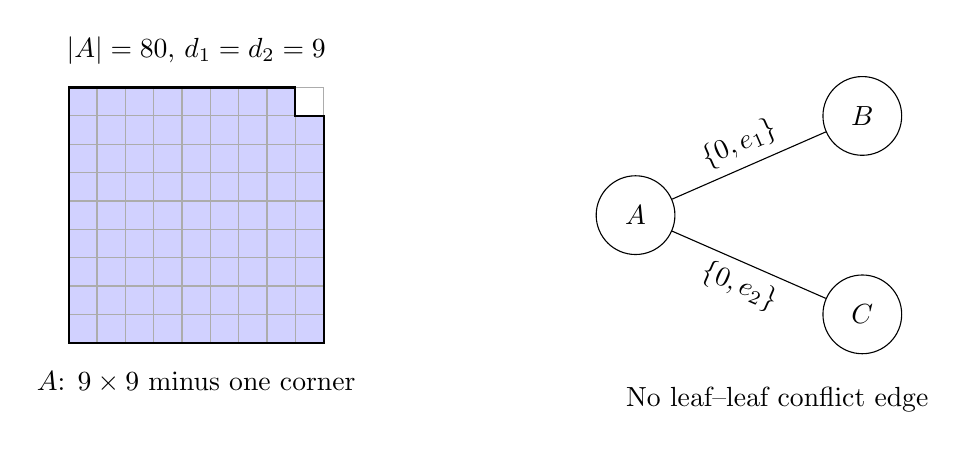
\begin{tikzpicture}[scale=.36]
 \fill[blue!18] (0,0) rectangle (9,9);
 \fill[white] (8,8) rectangle (9,9);
 \draw[step=1,gray!65,thin] (0,0) grid (9,9);
 \draw[thick] (0,0)--(9,0)--(9,8)--(8,8)--(8,9)--(0,9)--cycle;
 \node at (4.5,-1.4) {$A$: $9\times9$ minus one corner};
 \node at (4.5,10.3) {$|A|=80$, $d_1=d_2=9$};
 \node[draw,circle,minimum size=1cm] (a) at (20,4.5) {$A$};
 \node[draw,circle,minimum size=1cm] (b) at (28,8) {$B$};
 \node[draw,circle,minimum size=1cm] (c) at (28,1) {$C$};
 \draw (a)--node[above,sloped] {$\{0,e_1\}$}(b);
 \draw (a)--node[below,sloped] {$\{0,e_2\}$}(c);
 \node[align=center] at (25,-2) {No leaf--leaf conflict edge};
\end{tikzpicture}
\caption{An attaining center shape and the normalized two-voltage star.
The missing corner reduces $81$ to $80$ while preserving nine exits in each
direction.}
\end{figure}

\begin{remark}[General cyclic size; mathematical proof only]\label{rem:general}
The proofs of Lemma~\ref{lem:minority} and Theorem~\ref{thm:region}
work with $169,13$ replaced by $p^2,p$ on $(\Z/p\Z)^2$.
For odd $p\ge3$, the largest common guaranteed occupancy is consequently
the largest integer $k$ with
\[
 2k+\lceil\sqrt{k}\rceil\le p^2.
\]
Indeed, writing $t=p^2-2k$, a compatible triple with sizes at least $k$
has $k\le |A|\le p^2-k$. If $t<p$, the directional minority bound
gives $k\le t^2$; if $t\ge p$, the same inequality follows from
$k\le p^2$. Thus $\lceil\sqrt{k}\rceil\le t$ is necessary. For
sufficiency use a $k$-cell Ferrers diagram in a square of side
$\lceil\sqrt{k}\rceil$, then the two dilation complements. For admissible
$k$ this square has side less than $p$ and each leaf has at least $k$
points. The cyclic and Ferrers Lean modules in this release specialize
to $p=13$; this general-$p$ observation is a hand-proved corollary, not a
claim of full parameterized formalization.
\end{remark}

\section{An actual three-fiber realization in \texorpdfstring{$C_{13}^{\boxtimes6}$}{C13\string^6}}
The mask constraints are not a hypothetical separation profile. We now
identify the actual finite graph on which they occur. All coordinates in
this section are modulo $13$. Define three maps $\phi_i:H\to H^3$,
viewing $H^3$ as six cycle coordinates, by
\begin{align}
 \phi_0(x,y)&=(x,2x,y,-2y,0,x),\nonumber\\
 \phi_1(x,y)&=(x-1,2x-1,y,-2y,0,x-1),\label{eq:physical}\\
 \phi_2(x,y)&=(x-1,2x-1,y,-2y+1,0,x+1).\nonumber
\end{align}
These are three gauge-shifted BPZ kernel fibers: the kernel is
$h(x,y)=(x,2x,y,-2y,0,x)$, and the syndrome labels in the upstream
encoding are $0,2197,2368$. Both leaf parameters have been translated
by $(-1,0)$ so that the directional constraints take the form
\eqref{eq:compat}.

\begin{lemma}[Exact physical conflict relation]\label{lem:physical}
The map $(i,z)\mapsto\phi_i(z)$ is injective on $\{0,1,2\}\times H$.
Each fiber is independent. Between different fibers, the only possible
closed-conflict pairs are
\begin{align*}
 \phi_0(z)\conf\phi_1(w)&\quad\Longleftrightarrow\quad z=w\ \text{or}\ z=w-e_1,\\
 \phi_0(z)\conf\phi_2(w)&\quad\Longleftrightarrow\quad z=w\ \text{or}\ z=w-e_2.
\end{align*}
There are no closed conflicts between the two leaf fibers.
\end{lemma}
\begin{proof}
For residues $\delta\in\Z/13\Z$, the simultaneous requirements
$\delta,2\delta\in\{0,1,-1\}$ imply $\delta=0$. Within one fiber,
the first two coordinates therefore force equal $x$, and the third
and fourth force equal $y$.

For a center--first-leaf pair, put $\delta=x-s$ and $\eta=y-t$.
The relevant differences are
$\delta+1,2\delta+1,\eta,-2\eta,0,\delta+1$.
They all lie in $\{0,1,-1\}$ exactly when $\eta=0$ and
$\delta\in\{-1,0\}$. For a center--second-leaf pair the sixth
difference is $\delta-1$, which, together with the first two,
forces $\delta=0$; the third and fourth are $\eta,-2\eta-1$,
forcing $\eta\in\{-1,0\}$. This proves the two displayed relations.

For a first-leaf--second-leaf pair, the first two differences are
$\delta,2\delta$, so closed conflict would force $\delta=0$;
the sixth difference is then $-2$, which is not confusable with zero.
Finally the invariants ``second minus twice first'' distinguish the
center from the leaves, and ``fourth plus twice third'' distinguish
the leaves from one another. Along with injectivity within each fiber,
these establish injectivity of the full $507$-point map.
\end{proof}

For masks define the physical set
\[
 \mathcal C(A,B,C)=\phi_0(A)\cup\phi_1(B)\cup\phi_2(C).
\]
\begin{theorem}[Graph form of the allocation region]\label{thm:actual}
Under all the hypotheses of Theorem~\ref{thm:region}, there are masks
whose physical union is independent, whose center fiber has exactly
$a$ points and whose leaf fibers have at least $b,c$ points, if and
only if $\min(a,169-a)\le uv$.
\end{theorem}
\begin{proof}
By Lemma~\ref{lem:physical}, independence of the physical union is
equivalent to~\eqref{eq:compat}. Injectivity identifies each physical
fiber cardinality with its mask cardinality. Apply
Theorem~\ref{thm:region} in both directions.
\end{proof}

Corollary~\ref{cor:80} thus gives an actual $240$-point independent set
in $C_{13}^{\boxtimes6}$. This realizes a balanced occupancy constraint,
not a capacity improvement: the two \emph{complete} leaves already form
an independent set of size $338$, and the retained $522$-dimensional
construction has a much larger normalized root. The utility of the
theorem is its exact answer when a surrounding problem prescribes
joint local occupancies. An insertion into a larger fiber code would
still require separation from all outside fibers. No such global
gluing or resulting gain is established here.

\section{Contextual capacity certificates}\label{sec:capacity}
We include two previously completed actual-code certificates. This
section describes how their sets are constructed and how their exact
roots compare to the fixed prior constructions. Their finite recipes
are in the companion, and their formal endpoints are imported unchanged.

\subsection{The 300-dimensional \texorpdfstring{$C_7$}{C7} construction}
A private-pair gadget consists of an independent main code $I$, selected
pairs $(r_j,q_j)$ with all endpoints distinct, $r_j\in I$, $q_j\notin I$ and
$\Nb(q_j)\cap I=\{r_j\}$, two independent complementary ordered
transversals $P^{\rm H},P^{\rm V}$, and an independent auxiliary set $X$
avoiding their \emph{common} neighborhood. Let $R=\{r_j\}$ and
$B=I\setminus R$. The auxiliary partition is
\[
 X^0=X\setminus(\Nb(P^{\rm H})\cup\Nb(P^{\rm V})),\quad
 X^{\rm H}=X\cap\Nb(P^{\rm H}),\quad
 X^{\rm V}=X\cap\Nb(P^{\rm V}).
\]
Its profile is $(a,t,s,o,h,v)=(|I|,|R|,|X|,|X^0|,|X^{\rm H}|,|X^{\rm V}|)$.
The five-dimensional BPZ leaf has profile $(367,8,367,322,26,19)$.

In the ordinary paper routing, the Gao product's main code is the union
of seven separated blocks
\begin{align*}
 I'={}&B_L\times B_R\ \cup R_L\times X_R^0
 \ \cup P_L^{\rm H}\times X_R^{\rm H}
 \ \cup P_L^{\rm V}\times X_R^{\rm V}\\
 &\cup X_L^0\times R_R
 \ \cup X_L^{\rm H}\times P_R^{\rm V}
 \ \cup X_L^{\rm V}\times P_R^{\rm H}.
\end{align*}
Its private endpoints and ordered transversals are obtained by extending
left private pairs over $X_R^0$ and right private pairs over $X_L^0$.
For example,
$P'^{\rm H}=(P_L^{\rm H}\times X_R^0)\cup(X_L^0\times P_R^{\rm V})$.
The ordinary auxiliary set is $X_L\times X_R$.
The upstream Lean routing is the operation
\code{liftRPS S (flip T)} for this paper's $\Gao(S,T)$; the right flip
is essential to the identification.

Tandon's heterogeneous step keeps that main code, private-pair data
and ordered transversals but replaces the auxiliary set by
\begin{equation}\label{eq:hetero}
 X'=(J_0\times X_R^0)\,\dot\cup\,
     (J_H\times X_R^{\rm H})\,\dot\cup\,
     (J_V\times X_R^{\rm V}).
\end{equation}
Here each $J$ is independent and $J_0$ avoids the common neighborhood
of the left transversals. Right-side class separation makes the three
blocks independent and mutually separated. If
$q_H=|J_H\setminus\Nb(X_L^0)|$, $q_V=|J_V\setminus\Nb(X_L^0)|$
and $(s_0,o_0,h_0,v_0)$ describes $J_0$ relative to the actual left
transversals, then
\begin{align}
 s'&=s_0o_R+|J_H|h_R+|J_V|v_R,\nonumber\\
 o'&=o_0o_R+q_Hh_R+q_Vv_R,\label{eq:hetprofile}\\
 h'&=h_0o_R+(|J_V|-q_V)v_R,\nonumber\\
 v'&=v_0o_R+(|J_H|-q_H)h_R.\nonumber
\end{align}
The main-code and pair counts remain
$a'=(a_L-t_L)(a_R-t_R)+t_Ls_R+s_Lt_R$ and
$t'=t_Lo_R+o_Lt_R$. Thus an unchanged current main code can still
carry a more useful downstream auxiliary geometry.

For the same ordered inputs, ordinary and heterogeneous products are
actual siblings: their $I$, ports and ordered endpoint maps are
identical, not merely equicardinal. This justifies using one sibling's
auxiliary set as another's $J_0$. It does \emph{not} identify their
neutral sets. In~\eqref{eq:hetprofile}, ``outside'' always means outside
the \emph{closed neighborhood of the host's $X_L^0$}, never outside
just its endpoint set.

The accepted finite side counts used by this construction are:
\begin{center}\small
\begin{tabular}{@{}llllr@{}}
\toprule
 & Side set & Neutral reference & Side size & Outside count\\
\midrule
C1 & $J^+$ & $G_{10}.X^0$ & $134753$ & $27488$\\
C2 & $J_{15}$ & $G_{15}^{X}.X^0$ & $49495055$ & $12839823$\\
C3 & $G_{15}^{\rm het}.X$ & $G_{15}^{X}.X^0$ & $49433743$ & $14045805$\\
C4 & $J_{30}^{++}$ & $L_{30}.X^0$ & $2455726444728097$ & $841760069965664$\\
\bottomrule
\end{tabular}
\end{center}
Here $J^+$ is an automorphic ten-dimensional code with eight same-size
exchanges, $J_{15}$ is an automorphic ordinary fifteen-dimensional
code, and $J_{30}^{++}$ is an automorphic code obtained from two
$G_{15}^{\rm het}$ inputs. All their literal data and identities are
included in the Lean dependencies; these numbers are not assumed
profiles. In particular C4 refers to the ordinary $L_{30}$, not its
modified auxiliary sibling.

For completeness the compressed counting principle is as follows.
Write a source as a disjoint union of products and a reference as a
union of products. For each source factor, record a Boolean vector
of membership in the closed neighborhoods of all reference factors,
together with the exact frequency of each vector. On concatenating
coordinates take componentwise conjunction and multiply frequencies;
sum frequencies that yield the same vector. The all-false final vector
counts exactly the points outside the reference neighborhood, since
neighborhoods of products factor coordinatewise. Summing over the
disjoint source blocks gives the whole count. The Lean implementation
links its finite lookup tables and bitset operations to this actual
graph predicate.

The seven-family realization associated to a gadget is
\[
 \PhiG(G)=(B,N,A,D,O,H,V)
 =(I\setminus R,X^0,X^{\rm V},X^{\rm H},R,P^{\rm H},P^{\rm V}).
\]
Each family is independent and the required separated pairs are
\begin{equation}\label{eq:letters}
 BO,\ BH,\ BV,\ NA,\ ND,\ NO,\ NH,\ NV,\ AD,\ AH,\ DV.
\end{equation}
When literal label words have a separating pair in some coordinate,
their physical product blocks are independent and disjoint. Their
union has exact size
\begin{equation}\label{eq:weighted}
 W_K(w_1,\ldots,w_r)=\sum_{z\in K}\prod_{i=1}^r w_i(z_i).
\end{equation}
This is the BPZ layered substitution principle, not a numeric-only
profile propagation rule.

The retained strong construction makes three auxiliary refinements,
at dimensions $15$, $30$ and $40$, using genuine sibling identities.
The resulting forty-dimensional gadget has seven-family weights
\begin{align*}
 (&305594401588752181313,\ 175215226049998841399,\\
  &89250516720400951188,\ 65106977219472028790,\\
  &26158021392280384832,\ 26158021392280384832,\
    26158021392280384832).
\end{align*}
Use this realization and two copies of the inherited flipped
fifty-five-dimensional realization in BPZ's $S_{3b}$ substitution.
The output has dimension $150$. Apply to two copies the terminal code
\[
 K_2=\{BB,HN,NH,HD,VA,DV,AH\}.
\]
Its seven words are pairwise separated under~\eqref{eq:letters}. For
an identical input vector $(b,n,a,d,0,t,t)$ its weight is
$b^2+2t(n+a+d)$. Equation~\eqref{eq:weighted} therefore gives an
actual $300$-dimensional code of size $M_{300}$, recorded in
Appendix~\ref{app:integers}. The full dependency recipe, not just the
top weights, accompanies the source.

\begin{theorem}[Retained $C_7$ certificate]\label{thm:c7}
There is a code in $C_7^{\boxtimes300}$ of size $M_{300}$, and
\[
 3258834805519757^{300}<M_{300}(10^{15})^{300}.
\]
Consequently $\Theta(C_7)>3.258834805519757$.
\end{theorem}
\begin{proof}
The actual gadget and sibling identities establish the input
realizations; the certified $S_{3b}$ and $K_2$ tables establish
independence and the exact weighted cardinality. The finite integer
inequality is part of the accepted Lean certificate. Taking positive
$300$th roots and using the defining capacity lower bound proves
the strict endpoint.
\end{proof}

The companion also retains the $280$-dimensional simple terminal size
$M_{280}$. Its selected prior $560$-dimensional Stavriianov certificate
has size $M_{\rm S}=M_{280}^2$; this is an exact identity between the
listed integers, not an equality of capacities. The accepted comparison
$M_{280}^{300}<M_{300}^{280}$ gives
\[
 M_{\rm S}^{15}<M_{300}^{28},\qquad
 M_{\rm S}^{1/560}<M_{300}^{1/300}.
\]
The earlier Tandon $500$-dimensional root is also exceeded, but Table~\ref{tab:roots}
uses the stronger chosen prior root.

\subsection{The guarded 522-dimensional \texorpdfstring{$C_{13}$}{C13} construction}
The construction uses Protti's $58$ typed actual base cells, each
formed from explicit BPZ syndrome fibers. Their independence, required
separations and cardinalities are proved using the actual sets
\code{BaseC13.Pre}. They are not formal letters whose sizes are
postulated. Long's $49$-node recursion DAG, input orientations and
$K_{3a}$ terminal are retained. The only additions are the following
guarded reference words, with child order part of the definition:
\begin{center}\small
\begin{tabular}{@{}llllr@{}}
\toprule
Node & Ordered children & Output & References & Added typed cells\\
\midrule
$n_{12}$ & $n_6,n_{10},n_{11}$ & $A$ & $BAB,BBV$ & $6$\\
$n_{16}$ & $n_{11},n_{14},n_{15}$ & $A$ & $BAB,BBV$ & $3$\\
$n_{36}$ & $n_{35},n_9,n_{21}$ & $A$ & $BAB,BBV$ & $3$\\
$n_{17}$ & $n_5,n_{12},n_{16}$ & $N$ & $BBA,BBH,BVB,VAB,VBH,VHB$ & $15$\\
$n_{37}$ & $n_{20},n_{34},n_{36}$ & $N$ & same six words & $21$\\
\bottomrule
\end{tabular}
\end{center}
The final typed tables contain $4460$ generator words and $300$
terminal words. The terminal children are $n_{17},n_{37},n_{48}$,
of block dimensions $34,36,17$: in actual cycle coordinates the
dimension is $6(34+36+17)=522$.

A type records the required avoidance relations with output families.
After a child changes, masks are recomputed for that actual child
context. The chosen extension cells avoid the output and its required
neighbors, while retained cells acquire conservative mask bits.
Literal rows certify internal independence, required cross-row
separation and absence of duplicate generator words. These statements
build actual \code{Realisation.multiSubst} objects. Their cardinality
identities come from~\eqref{eq:weighted}; repeated occurrences of a
shared DAG child use \emph{new coordinate blocks}, so sharing is not
physical coordinate reuse. The flattening graph isomorphism gives a
finite code in the actual cycle strong power.

Joint additions need not have monotone downstream gains: an enlarged
child avoidance mask can shrink later usable cells. This is why the
accepted final tables are those for the complete chosen combination,
not independent increases of scalar intermediate profiles.

\begin{theorem}[Retained $C_{13}$ certificate]\label{thm:c13}
There is an independent set of size $N_{522}$ in
$C_{13}^{\boxtimes522}$. If $M_{\rm L}$ is Long's fixed $522$-dimensional
certificate size, then
\[
 N_{522}>M_{\rm L},\qquad
 6302927403571109^{522}<N_{522}(10^{15})^{522}.
\]
In particular $N_{522}^{1/522}>M_{\rm L}^{1/522}$ and
$\Theta(C_{13})>6.302927403571109$.
\end{theorem}
\begin{proof}
The typed base realization, checked substitutions and terminal code
construct the actual independent set. Their proved weighted identities
give its cardinality $N_{522}$. The two exact integer comparisons are
in the accepted capacity and strict-display modules. Monotonicity of
positive $522$th roots and the code-to-capacity inequality prove both
claims. Both full integers appear in Appendix~\ref{app:integers}.
\end{proof}

The new local region is logically separate from this certificate:
the masks of Sections~2--4 have not been glued into its full DAG or
base fibers. Neither strict endpoint changed in the structural round.

\section{Formal statements, trust and reproduction}\label{sec:formal}
The project pins Lean $4.32.2$ and mathlib revision
\begin{center}\small\texttt{905b95818eb32af7874a58b427f50c1711a5e96c}.\end{center}
Only selected transitive local imports are bundled. BPZ, Long and
Protti source headers and Apache-2.0 licensing are retained; mathlib
is an external dependency. The following map identifies the endpoints
used by the mathematical claims:
\begin{center}\small
\begin{tabular}{@{}>{\raggedright\arraybackslash}p{.37\textwidth}>{\raggedright\arraybackslash}p{.58\textwidth}@{}}
\toprule
Claim & Module and declaration\\
\midrule
Minority rectangle & \code{MinorityRectangle}: \code{minority_rectangle}\\
Exact abstract region & \code{StarRegion}: \code{star_region_iff}\\
Actual graph region & \code{ActualRegion}: \code{actual_star_region_iff}\\
Balanced optimum and $240$ points & \code{ActualRegion}: \code{actual_star_upper80},
 \code{actual_star_attains80}; \code{PhysicalStar}: \code{cycleCode_independent},
 \code{cycleCode_card}\\
$C_7$ strict endpoint & \code{C7Improvement.Capacity}:\newline
 \code{shannonCapacity_C7_gt_strong}\\
$C_{13}$ strict endpoint & \code{ExplorationC13FrontierR03.StrictDisplay}:
 \code{strict_capacity_lower}\\
Classical $C_7$ illustration & \code{ExplorationC7.Correlated.Geometry},
 \code{ExplorationC7.Correlated.Witness}\\
\bottomrule
\end{tabular}
\end{center}
The new aliases \code{StructuralRelease.c7_strict},
\code{c13_strict}, \code{c13_region}, \code{c13_example} and
\code{c7_illustration} preserve these statement types. In particular
\code{c13_region} retains both pair budgets, both strict slack
hypotheses, exact center size and lower-bound leaf sizes.

The minority-rectangle argument is symbolic and uses standard logic.
The cyclic and Ferrers templates, literal construction tables, and
physical relation use \code{native_decide}. The physical check has $507$ points.
This adds compiler trust; it is not advertised as purely kernel
arithmetic. The accepted audits report $62$ native dependencies in
the selected strong $C_7$ strict closure; $166$ in the selected
$C_{13}$ endpoint union including strict display ($161$ new, $5$
upstream); $9$ in the eleven selected local structural declarations
($6$ new, $3$ BPZ); and $8$ in twenty selected $C_7$ illustration
closures. The six-declaration historical $C_7$ audit union has $66$,
which is a different count from the single endpoint's $62$.
Otherwise the reported axioms are standard \code{propext},
\code{Classical.choice} and \code{Quot.sound}; the selected accepted
audits contain no holes or unexpected mathematical axioms.

The structural necessity proof ranges over \emph{arbitrary} masks.
Only the finite sufficiency templates are checked computationally:
\code{ferrers_statistics} verifies all $13\cdot13\cdot170$ parameter
triples satisfying the rectangle-size condition, including complement
templates. The physical relation check covers the $507$-point
three-fiber map, after which arbitrary compatible masks are handled
symbolically. This separates a finite certificate from its semantic
transport rather than assuming candidate densities.

For this publication we copied exact-source accepted compiled artifacts
locally and compiled \emph{only the new aggregate integration target}.
That validates imported statement types and coexistence of the selected
namespaces; it is not a fresh clean-clone execution of the original
large finite checks. Accepted audit reports are included as provenance,
not regenerated here. No old side counts, baseline audits or searches
were rerun. A reader's clean build executes those original finite
certificates from source:
\begin{verbatim}
cd lean
lake exe cache get
lake build StructuralRelease
\end{verbatim}
The README gives prerequisites, the logged reproduction wrapper and the
scope of the performed validation. Caches and compiled files are not
part of the release. The public repository is
\begin{center}\small
\url{https://github.com/JingzheShi/odd-cycle-shannon-structural-lean}.
\end{center}

\appendix
\section{Classical correlated separation in \texorpdfstring{$C_7^3$}{C7\string^3}}\label{app:c7}
For a complete rectangle $\mathcal R(P)=\prod_i P_i$ one has
\begin{equation}\label{eq:rectangle}
 \mathcal R(P)\sep\mathcal R(Q)
 \quad\Longleftrightarrow\quad
 \text{there is a coordinate $i$ with }P_i\sep Q_i.
\end{equation}
The reverse implication is immediate. For the other direction, if
each coordinate fails separation, choose one confusable pair there;
their concatenations are a confusable pair of rectangle points.
This proof also handles empty factors, whose separation is vacuous.
For arbitrary correlated sets the exact criterion instead is
\begin{equation}\label{eq:routed}
 S\sep T\quad\Longleftrightarrow\quad
 \forall x\in S\ \forall y\in T\ \exists i:
 x_i\not\conf y_i.
\end{equation}
The separating coordinate may depend on the pair. These are classical
strong-product and graph-packing principles; complement-homomorphism
and packing treatments give the wider context \cite{sauer,zuiddam}.

Here is a literal, nonaffine example:
\begin{align*}
 P={}&\{(0,0,0),(1,2,1),(2,4,2),(3,6,3),\\
     &\hspace{8mm}(4,1,4),(5,5,5),(6,3,6)\},\\
 Q={}&\{(0,0,2),(1,1,4),(2,2,6),(3,4,0),\\
     &\hspace{8mm}(4,3,5),(5,6,1),(6,5,3)\}.
\end{align*}
Both sets are independent, $P\sep Q$, and each coordinate image of
each set is all of $\Z/7\Z$. Thus their rectangular hulls both equal
the entire $343$-point ambient space, so no universal separating
coordinate exists. Their second-coordinate permutations are not of
the form $x\mapsto ax+b$: in $P$ the entries at $0,1$ force
$b=0,a=2$, inconsistent with the entry at $5$; in $Q$ they force
$b=0,a=1$, inconsistent with the entry at $3$.

Each of the three coordinates is essential for the stated $P/Q$
separation, as the following pairs are nonconfusable in exactly the
listed coordinate:
\begin{center}
\begin{tabular}{@{}cll@{}}\toprule
Only separating coordinate & Point of $P$ & Point of $Q$\\\midrule
$0$ & $(0,0,0)$ & $(5,6,1)$\\
$1$ & $(1,2,1)$ & $(0,0,2)$\\
$2$ & $(0,0,0)$ & $(0,0,2)$\\\bottomrule
\end{tabular}
\end{center}
Deleting any coordinate makes the corresponding pair confusable.
More generally a projection obtained only by deleting or repeating
coordinates can preserve this separation only if its coordinate map
is surjective onto all three original coordinates. This does not
restrict arbitrary recoding of the points.

The two whole blocks already fit BPZ's arbitrary \code{Realisation}
interface as two separated virtual letters; no new composition
machinery is needed. The literal witness and its graph claims are
formalized, but its $14$ points are fewer than the simple product's
$3^3=27$. One completed fixed-context test on the $78$ points outside
the closed neighborhood of $P\cup Q$ explored $4652$ search nodes
and retained at best $27$ points. That recorded result concerns only
this particular completion problem, not every correlated code and
not $\Theta(C_7)$. No capacity gain or new lower-bound mechanism is
claimed for the illustration.

\section{Exact certificate integers}\label{app:integers}
The following displays denote decimal concatenation of their lines;
line breaks are not multiplication. These integers also appear as
literal definitions in the corresponding Lean modules and as decimal
strings in \code{data/exact_roots.json}. $M_{280}$ identifies the
chosen Stavriianov integer through $M_{\rm S}=M_{280}^2$.
\[
M_{280}=\left[\begin{array}{l}
\mathtt{454402134191994507126819903596564906706672995987342041247384}\\
\mathtt{728314329074657273274845475279319219681718758139567086979352}\\
\mathtt{344706380862194486578561}
\end{array}\right]_{\rm concat}.
\]

\[
M_{300}=\left[\begin{array}{l}
\mathtt{829285028795068306996156269127051491792580794837082180052404}\\
\mathtt{457654405642151270168458082344281085433541502968490704472521}\\
\mathtt{4369985043992527534955657521950273}
\end{array}\right]_{\rm concat}.
\]

\[
N_{522}=\left[\begin{array}{l}
\mathtt{229658862260924106595253952272045722516666849084998891003074}\\
\mathtt{565947208437477777984843267498257757027599220802987164115637}\\
\mathtt{395623399737872969052176585212885966843594415072366106347620}\\
\mathtt{633527919020308823654200143088901344335953552868018939685799}\\
\mathtt{436735561005316491462893882696633487887255686360035537551619}\\
\mathtt{671849877807457341677220644469448879804632334817769471949487}\\
\mathtt{8137521970969100483646258158547494769299673652709061296128}
\end{array}\right]_{\rm concat}.
\]

\[
M_{\rm L}=\left[\begin{array}{l}
\mathtt{229652548049794108669807110452510507772003551488435507257929}\\
\mathtt{181011771863281382028370787610380986376743189829161636850800}\\
\mathtt{135155371587104528625458030017679021783209914609549343731326}\\
\mathtt{915703357857186485927010917180050856575156133657818150496082}\\
\mathtt{954825607329536419413840822416591512368164009868691426795406}\\
\mathtt{198331457870964794955825596500475143546966222926330319233036}\\
\mathtt{5907306254086949021017927545131180608697270602131050594304}
\end{array}\right]_{\rm concat}.
\]


\begin{thebibliography}{12}
\raggedright
\bibitem{gao} Yu Gao.
\emph{A Recursive Construction Improving the Lower Bound on the Shannon
Capacity of $C_7$}. arXiv:2607.27869v1, 2026.
\bibitem{bpz} Pjotr Buys, Sven Polak and Jeroen Zuiddam.
\emph{Lean-verified lower bounds for the Shannon capacity of odd cycles}.
arXiv:2607.29681v1, 2026.
\bibitem{bpzcode} Buys, Polak and Zuiddam.
\emph{shannon-capacity-lean}, Apache-2.0 source, revision
\texttt{aa21eeb12b75b0413d3fa9fb4208b5d0bf2c4d65}.
\url{https://github.com/spectra-research/shannon-capacity-lean}.
\bibitem{tandon} Ravi Tandon.
\emph{Strengthening Recursive Constructions for Zero-Error Shannon
Capacity}. arXiv:2608.30273v1, 2026. Theorem~1 and Section~4.2.
Companion \emph{C7-Shannon-Capacity-Heterogeneous-Recursion}, Apache-2.0.
\bibitem{protti} Matthew Protti.
\emph{Checked Shannon constructions and canonical cell retyping}.
\emph{c11-shannon-capacity-lower-bound}, release v0.5.0, 2026,
Apache-2.0 source, revision
\texttt{dfaef37e60e55c55b1744d9badd1f26c5364c7d5}.
\url{https://github.com/matthewprotti/c11-shannon-capacity-lower-bound}.
\bibitem{long} Griffin Long.
\emph{shannon-capacity-c15-c19}, release v1.1, 2026, Apache-2.0
source, revision \texttt{a06e1a19278852350eb912c585adf0888fb54b91}.
\url{https://github.com/griffinwork40/shannon-capacity-c15-c19}.
\bibitem{stav} Oleksii Stavriianov.
\emph{Searching the recursion tree improves the lower bound on the
Shannon capacity of $C_7$}. Release 1.0.3, 2026,
doi:10.5281/zenodo.22728595. Revision
\texttt{577c73e967531a77c8adde2bb71fd99656435c4c}.
\url{https://github.com/Ratatosk32/c7-recursion-tree}.
\bibitem{grid} B\'ela Bollob\'as and Imre Leader.
Edge-isoperimetric inequalities in the grid.
\emph{Combinatorica} 11(4), 299--314, 1991.
doi:10.1007/BF01275667.
\bibitem{torus} B\'ela Bollob\'as and Imre Leader.
An isoperimetric inequality on the discrete torus.
\emph{SIAM Journal on Discrete Mathematics} 3(1), 32--37, 1990.
doi:10.1137/0403004.
\bibitem{sauer} Norbert Sauer and Joel Spencer.
Edge disjoint placement of graphs.
\emph{Journal of Combinatorial Theory, Series B} 25(3), 295--302, 1978.
doi:10.1016/0095-8956(78)90005-9.
\bibitem{zuiddam} Jeroen Zuiddam.
The asymptotic spectrum of graphs and the Shannon capacity.
\emph{Combinatorica}, 2019. arXiv:1807.00169v2.
doi:10.1007/s00493-019-3992-5.
\end{thebibliography}
\end{document}
